\documentclass{article}
\linespread{0.7}
\usepackage[a4paper, margin=3mm, landscape]{geometry}
\usepackage{multicol}
\usepackage{xcolor}
\usepackage{enumitem}
\usepackage{amsmath}
\usepackage{amsfonts}
\usepackage{listings}
\usepackage{soul}
\usepackage{graphicx}

\pdfinfo{
    /Title (template.pdf)
    /Creator (TeX)
    /Producer (pdfTeX 1.40.0)
    /Author (securespider)
    /Subject (template)
    /Keywords (cheatsheet, pdf)
}

\graphicspath{ {./img/} }

\pagestyle{empty}
\setcounter{secnumdepth}{0}
\setlength{\columnseprule}{0.25pt}

% Redefine section commands to use less space
\makeatletter
\renewcommand{\section}{\@startsection{section}{1}{0mm}%
    {-1ex plus -.5ex minus -.2ex}%
    {0.5ex plus .2ex}%x
{\normalfont\large\bfseries}}
\renewcommand{\subsection}{\@startsection{subsection}{2}{0mm}%
    {-1explus -.5ex minus -.2ex}%
    {0.5ex plus .2ex}%
{\normalfont\normalsize\bfseries}}
\renewcommand{\subsubsection}{\@startsection{subsubsection}{3}{0mm}%
    {-1ex plus -.5ex minus -.2ex}%
    {1ex plus .2ex}%
{\normalfont\small\bfseries}}%
\makeatother

% Adjust spacing for all itemize/enumerate
\setlength{\leftmargini}{0.5cm}
\setlength{\leftmarginii}{0.5cm}
\setlist[itemize,1]{leftmargin=2mm,labelindent=1mm,labelsep=1mm}
\setlist[itemize,2]{leftmargin=2mm,labelindent=1mm,labelsep=1mm}

% Font
\renewcommand{\familydefault}{\sfdefault}

% Define colors for math formulas
\definecolor{myblue}{cmyk}{1,.72,0,.38}
\everymath\expandafter{\the\everymath \color{myblue}}

% Custom command for keywords
\definecolor{highlight}{RGB}{251,243,218}
\newcommand{\keyword}[2][]{\sethlcolor{highlight}\hl{\textbf{#2}} #1 - }
\newcommand{\ilkeyword}[1]{\sethlcolor{highlight}\hl{\textbf{#1}}}

% Define colors and style for code
\definecolor{codegreen}{rgb}{0,0.6,0}
\definecolor{codegray}{rgb}{0.5,0.5,0.5}
\definecolor{codered}{HTML}{CC241D}
\definecolor{backcolor}{rgb}{0.95,0.95,0.95}
\lstdefinestyle{codestyle}{
    backgroundcolor = \color{backcolor},
    commentstyle = \color{codegray},
    keywordstyle = \color{codered},
    stringstyle = \color{codegreen},
    basicstyle = \ttfamily,
    breakatwhitespace = false,
    showstringspaces = false,
    breaklines = true,
    showtabs = false,
    tabsize = 2
}
\lstset{style = codestyle}

% -----------------------------------------------------------------------
\begin{document}
\begin{multicols*}{3}
\footnotesize

% Title box
\begin{center}
    \fbox{
        \parbox{0.8\linewidth}{
            \centering \textcolor{black}{
                {\Large\textbf{CS3230}} \\
                \normalsize{Design and Analysis of Algorithms}} \\
                {\footnotesize \textcolor{gray}{github.com/securespider}}
        }
    }
\end{center}
\section{01. Stable matching}
Both sides rank each other and goal is to pair each up
\textbf{Constraints}
No \keyword{rogue couples}{matched partner likes someone more than current partner that also likes them back}
\subsection{Gale-Shapley Algo}
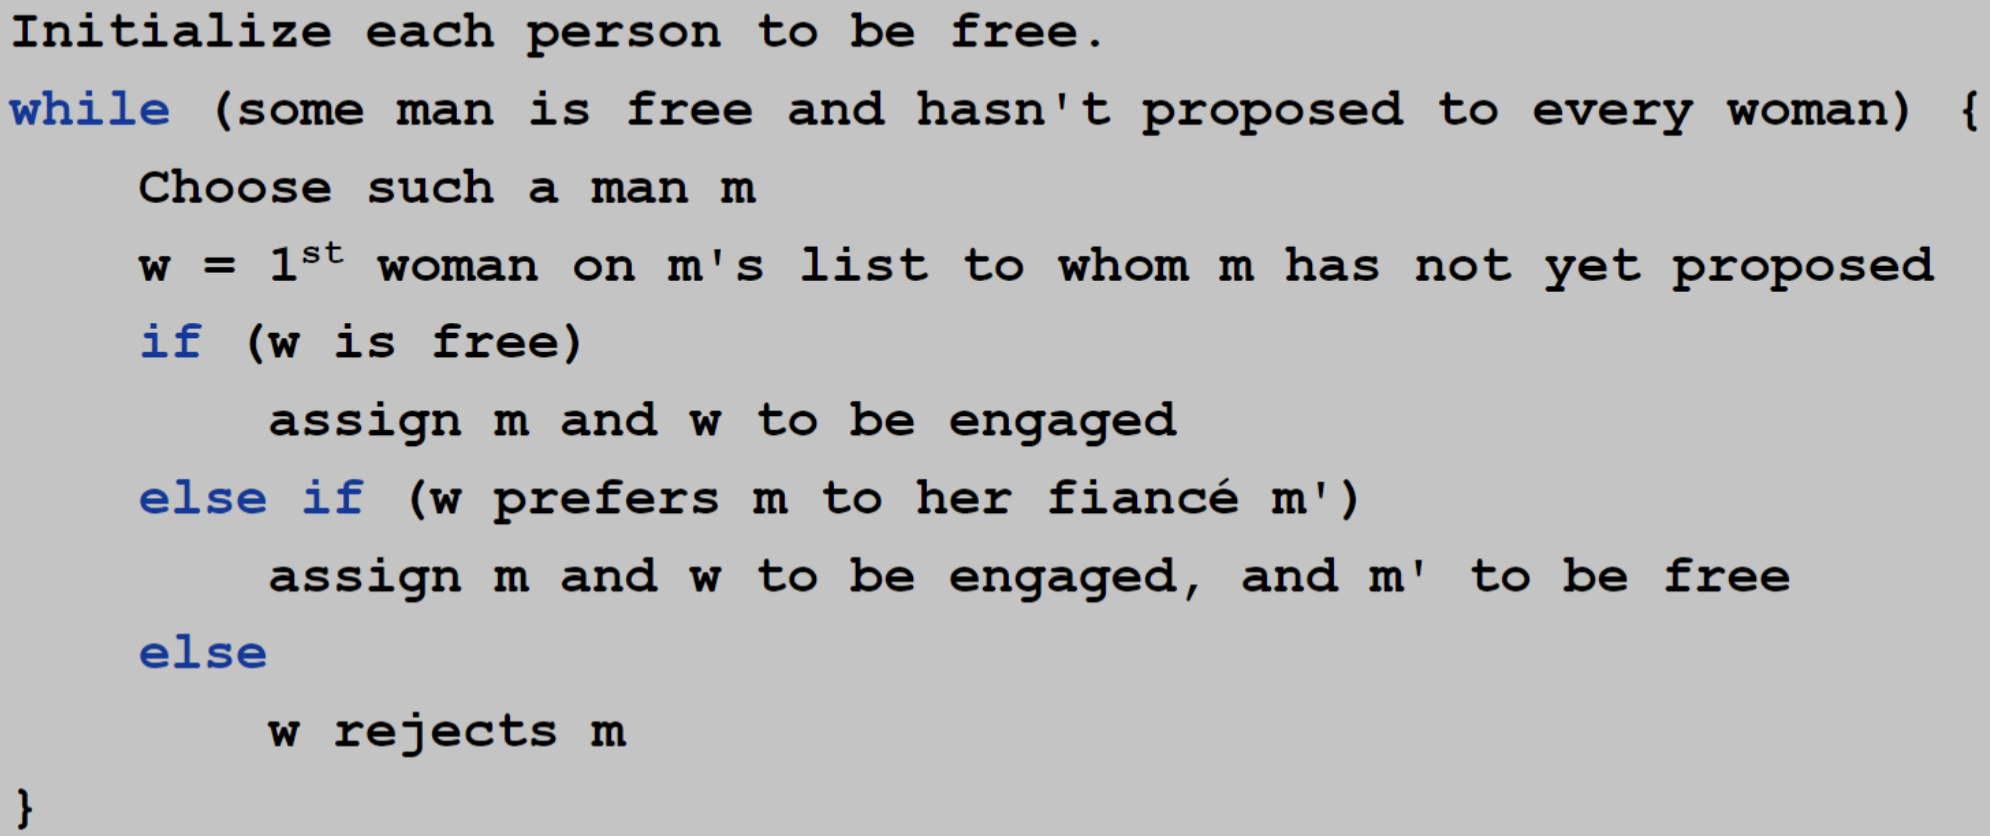
\includegraphics[scale=0.2]{01-gale-shapley-algo}
\subsubsection{Invariant}
\begin{itemize}
	\item If woman not on boy list, she has a better current fav
	\item Boy choice is strictly worsening
	\item Girl choice cannot worsen (weakly increasing)
\end{itemize}
\section{02. Algorithm Analysis}
\begin{description}
	\item[Algorithm]{Finite sequence of well-defined instruction to solve computational problem}
	\begin{itemize}
		\item Optimize running time
		\item Runtime is machine and input dependent
	\end{itemize}
\end{description}
\subsection{Word-RAM model}
\begin{itemize}
    \item Word is basic unit of memory (few bytes)
	\item Runtime $\approx$ number of instructions taken
	\item Ram can be accessed in the same time irrespective of location
	\item Every operation involves constant number of words and cycles by CPU
\end{itemize}
\subsubsection{Problem vs Algorithm}
\begin{itemize}
	\item Problem does not specify approach but algorithm defines ways/methods to solve prob
\end{itemize}
\subsection{Polynomial time}
\begin{itemize}
	\item There exist constants $c,d\in\mathbb{R}$ on every input of size N such that its running time is bounded by $cN^d$
	\item Brute Force - Checks all possible solution and typically takes exponential time $2^N$
	\item Generally efficient because c and d are low
\end{itemize}
\subsubsection{Worst-Case Analysis}
\begin{itemize}
	\item Bound on largest possible running of algorithm on input
	\item Captures efficiency in practice 
\end{itemize}
vs Average case running time
\begin{itemize}
	\item Hard to accurately model real instances by random distributions
	\item Tuned for certain distributions
\end{itemize}
\subsection{Asymptotic Order of Growth}
\begin{itemize}
	\item Compare for asymptotically large values of input sizes (rate of growth)
	\item Suppress constant factor and lower-order terms
\end{itemize}
\subsubsection{Bounds}
\begin{description}
	\item[Upper Bound]{T(n) = O(f(n)): Exist constants $c,n_o\geq 0$ such that $\forall n\geq n_0$, we have $T(n)\leq cf(n)$}
	\item[Lower Bound]{T(n) = $\omega$(f(n)): Exist constants $c,n_o\geq 0$ such that $\forall n\geq n_0$, we have $T(n)\geq cf(n)$}
	\item[Tight Bound]{T(n) = $\theta$(f(n)): T(n) is both O(f(n)) and $\omega$(f(n))}
\end{description}
\subsubsection{Properties}
\begin{description}
	\item[Transitivity]{If f = O(g) and g = O(h) then f = O(h)}
	\item[Additivity]{If f = O(h) and g = O(h) then f + g = O(h)}
\end{description}
\subsubsection{Bounds for some functions}
\begin{itemize}
	\item Polynomials - Just take the highest power
	\item Logarithms - Base doesn't matter and always smaller than polynomial
	\item Exponential - Always grows faster than polynomial
\end{itemize}
\subsection{Common runtimes}
\begin{itemize}
	\item O(n) - List traversal or merging lists
	\item nlogn - sorting, intervals, divide and conquer algos (recursive)
	\item $n^2$ - Finding pairs of elements
	\item $n^k$ - Enumerate subsets of k nodes, set disjoints
	\item Exponential - All subsets
	
\end{itemize}



\section{03. Graph}
\begin{itemize}
	\item Describes relationships between nodes/entities
\end{itemize}
\subsection{Representation}
\begin{description}
	\item[Adjacency Matrix]{$NxN$ matrix where $A_uv=$<weight> if (u,v) is an edge}
	\begin{itemize}
		\item Good for big graphs/a lot of edges(dense)
		\item O(1) time for checking edge
		\item Space is O($n^2$)
		\item Identifying all edges take O($n^2$) time
	\end{itemize}
	\item[Adjacency list]{List of linked lists representing nodes that are attached to each node}
	\begin{itemize}
		\item Good for sparse graphs/trees
		\item O(deg(u)) for checking edge
		\item Space is V+E
		\item Identifying all edges takes O(V+E) time
	\end{itemize}
\end{description}
\subsection{Path and Connectivity}
\begin{itemize}
	\item \keyword{Path}{Sequence P$\in \{v_0, v..v_k\}$ of nodes such that each adjacent pair is joined by an edge}
	\begin{description}
		\item[Simple]{All nodes are distinct}
		\item[Cycle]{Path such that $v_0=v_k, k>2$ and first k-1 nodes are distinct}
	\end{description}
	\item \keyword{Connected}{There is a path for all pairs of nodes}
	\item \keyword{Tree}{Undirected connected graph that does not contain a cycle}
	\begin{itemize}
		\item Any 2 implies Tree
		\item G is connected
		\item G does not contain cycle
		\item G has n-1 edges
	\end{itemize}
	\item \keyword{Rooted tree}{Arrangement of tree such that root is top and nodes attached to parent is in different level}
\end{itemize}
\subsubsection{Connectivity problems}
\begin{description}
	\item[s-t connectivity]{Is there path between any 2 points s, t}
	\item[s-t shortest path prob]{Length of shortest path btw s,t}
\end{description}
\subsection{Breadth First Search}
\subsubsection{Algorithm}
\begin{itemize}
	\item Explore outward from some node, s in all directions adding nodes one layer at a time
	\item Algorithm
	\begin{enumerate}
		\item Layer$_0$={s}
		\item $L_1$={neighbours of $L_0$}
		\item $L_n$ = {neighbours of $L_{n-1}$ not in all prev layers}
	\end{enumerate}
\end{itemize}
\subsubsection{Properties}
\begin{itemize}
	\item Induction theorem: $\forall i, L_i$ consist of nodes at dist(s) = i
	\item Let T be a BFS tree of $G = (V, E)$, and let $(x, y)$ be an edge of G. Then the level of x and y differ by at most 1.
	\item BFS runs in O(V+\# E) given adjacency list
\end{itemize}
\subsection{Bipartite graph}
\begin{itemize}
	\item Independent sets such that no nodes within the set are connected to each other but are connected to nodes of other sets
	\item Colour each node red or blue and every edge has strictly one red and blue end each
	\item Bipartite graphs cannot contain odd length cycles
\end{itemize}
\subsubsection{Algo for Bipartiteness}
\begin{itemize}
	\item Let G be a connected graph and $L_0..L_k$ are layers produced by BFS
\end{itemize}
\begin{enumerate}
	\item Edge between 2 nodes in same layer
	\begin{itemize}
		\item Graph is bipartite as we can colour alternate layers as red and blue
	\end{itemize}
	\item No edge btw nodes in same layer
	\begin{itemize}
		\item Graph cannot be bipartite as there is odd length cycle
		\item Let x,y be the 2 points in same level and has edge btw them
		\item Cycle: s-x-y-s (s-x == y-s) Odd length
	\end{itemize}
\end{enumerate}
\subsection{Directed graph}
\begin{itemize}
	\item Asymmetric edges: (u,v) (edge from u to v) does not imply (v,u) 
	\item Directed reachability problem: Find all nodes reachable from node s
\end{itemize}
\subsubsection{Strong Connectivity}
\begin{description}
	\item[Mutually reachable]{Path from u to v and vice versa}
	\item[Strongly connected]{Every pair of nodes are mutually reachable}
	\begin{itemize}
		\item Strongly connected iff every node reachable from s and s reachable from every node
	\end{itemize}
	\item[Algorithm]{Pick any node and run bfs on G and $G^{rev}$ (reverse orientation of every edge in G)}
	\begin{itemize}
		\item G is strongly connected if all nodes reached in both BFS executions
		\item Runs in O(m+n) time
	\end{itemize}
\end{description}
\subsection{Directed Acyclic Graph}
\begin{itemize}
	\item Directed graph that has no directed cycle
	\item \keyword{Precedence constraints}{Edge ($v_i, v_j$) means $v_i$ must preceed $v_j$}
	\item \keyword{Topological order}{For every edge ($v_i, v_j$) we have $i<j$}
	\begin{itemize}
		\item If G has a topological order, then G is a DAG (Proof by contra)
		\item If G is a DAG then G has a node without incoming edges (Proof contra)
	\end{itemize}
\end{itemize}


\section{04. Greedy algorithms}
\begin{itemize}
	\item Consider jobs in some order and immediately take the job that is compatible with the previous jobs
	\item Has some heuristic to sort the jobs
\end{itemize}
\subsection{Scheduling intervals}
\begin{itemize}
	\item Maximize number of jobs run
	\item Heuristic: \hl{end time}, start time, interval size, fewest conflict
\end{itemize}
\subsection{Interval Partitioning}
\begin{itemize}
	\item Minimize number of classrooms to run lectures concurrently
	\item Heuristic: \hl{start time}
	\item Assign lecture to first compatible classroom
\end{itemize}
\subsection{Minimize lateness scheduling}
\begin{itemize}
	\item Heuristic: \hl{Earliest deadline}, Shortest processing time first, Smallest slack ($d_j-t_j)$
	\item Start with an optimal solution and inductively reduce number of inversions until it reaches the greedy solution
\end{itemize}
\subsubsection{Inversions}
\begin{itemize}
	\item Pair of jobs i and j where dl(i)<dl(j) but j schedule before i
	\item Greedy solution does not have any inversions
\end{itemize}
\subsection{Greedy analysis Strategies}
\begin{enumerate}
	\item Each step in greedy solution is at least as good as other solutions
	\item Exchange argument: Transforming solution to greedy algorithm without hurting its quality
	\item Structural: Every solution has a certain value and greedy algos can be in this bound
\end{enumerate}
\subsection{Optimal offline caching}
\begin{itemize}
	\item Eviction strategy that minimises number of cache misses
	\item Note that the full sequence of requests is known a priori
	\begin{itemize}
			\item vs Online: Request not known in advance
	\end{itemize}
	\item Heuristic: \hl{Farthest in future}
	\begin{itemize}
		\item Evict item in cache that is not requested until farthest in the future
	\end{itemize}
\end{itemize}
\section{05. Divide and conquer algo}
\begin{itemize}
	\item Break up problem into several parts and sort each part recursively
	\item Combine solutions to sub-problems into overall solution
\end{itemize}
$$
T(n)\leq T(\lceil\dfrac{n}{2}\rceil)+T(\lfloor\dfrac{n}{2}\rfloor) + n
$$

\section{07. Network Flow}
\subsection{Minimum Cut/Max Flow Problem}
\subsubsection{Environment}
\begin{itemize}
	\item Directed graph with "capacity" as edge weights c(e)
	\item 2 nodes denoted as source and sink
\end{itemize}
\subsubsection{s-t cut}
\begin{itemize}
	\item Partition (A,B) of graph V with $s \in A$ and $t \in B$
	\item Capacity of a cut: $cap(A,B) = \sum_{edges out of A} c(e)$
\end{itemize}
\subsubsection{s-t flow}
\begin{itemize}
	\item Function that satisfies:
	\begin{itemize}
		\item $\forall e\in E 0 \leq f(e) \leq c(e)$
		\item $\forall v\in V - (s,t), \sum_{e in to V} = \sum_{e out of V} f(v)$
	\end{itemize}
	\item Value of flow: $v(f) = \sum_{e out of s} f(e)$
\end{itemize}
\subsubsection{Goals}
\begin{description}
	\item[Min s-t cut]{Find an s-t cut of minimum capacity}
	\item[Max s-t flow]{Find an s-t flow of maximum value}
\end{description}
\subsubsection{Flow Value Lemma}
\begin{itemize}
	\item Let f be any flow, and let (A,B) be any s-t cut. The net flow sent across the cut is equal to the amount leaving s
	$$\sum_{e out of A}f(e)-\sum_{e in to A}f(e)=v(f)$$
\end{itemize}
\subsubsection{Weak Duality}
\begin{itemize}
	\item Let f be any flow. Then for any s-t cut (A,B) we have $v(f)\leq cap(A,B)$
\end{itemize}
\subsubsection{Certificate of Optimality}
\begin{itemize}
	\item Let f be any flow and let (A,B) be any cut, if v(f) = cap(A,B) then f is a max flow and (A,B) is a min cut
\end{itemize}
\subsubsection{Residual Graph}
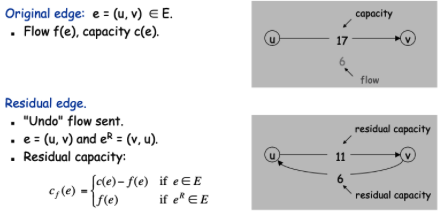
\includegraphics[scale=0.4]{07-residual-edge}
\begin{itemize}
	\item Residual graph is all residual edges with positive residual capacity
	\item $E_f=\{e:f(e) < c(e)\}\cup \{e^R:c(e) > 0\}$
\end{itemize}
\subsection{Ford Fulkerson}
\begin{enumerate}
	\item Find an augmenting path/flow 
	\begin{itemize}
		\item Can use BFS or DFS to find the path and get the bottleneck edge
		\item Flow value is the smallest value
		\item Keep track of the flow value
	\end{itemize}
	\item Augment the graph using residual edges
	\item Repeat until no feasible paths possible
\end{enumerate}
\subsubsection{Proof}
\begin{itemize}
	\item Flow f is a max flow iff there are no augmenting path
\end{itemize}
\begin{enumerate}[label=(\roman*)]
	\item There exists a cut (A,B) st v(f) = cap(A,B)
	\item Flow f is a max flow
	\item There is no augmenting path relative to f
\end{enumerate}
\begin{itemize}
	\item (i)-(ii): Corollary to weak duality to weak duality lemma
	\item (ii)-(iii): Contrapositive
	\begin{itemize}
		\item Suppose there exists an augmenting path, then we can improve flow by sending flow along path
	\end{itemize}
	\item (iii)-(i)
	\begin{enumerate}
		\item Let f be a flow with no augmenting path
		\item Let A be set of vertices reachable from s in residual path
		\item By definition of A, $s\in A$
		\item By definition of f, $t\notin A$
	\end{enumerate}
\end{itemize}
\subsubsection{Runtime}
\begin{itemize}
	\item All capacities are integers btw 1 and C
	\item Every flow value f(e) and every residual capacity remains an integer throughout the algorithm
	\item Algorithm terminates in at most $v(f^*)\leq nC$ iterations
	\begin{itemize}
		\item Each augmentation increase value by at least 1
	\end{itemize}
	\item If C = 1, Ford-Fulkerson runs in O(mn) time
	\item If all capacities are integers, then there exists a max flow f for which every flow value f(e) is an integer.
	\begin{itemize}
		\item Since algorithm terminates, theorum follows from point 2
	\end{itemize}
\end{itemize}
\end{multicols*}
\end{document}
